\section{Complete Performance and Ranking Context}\label{app:results}
\begin{table}[t]\centering\small
\caption{Equal-window source/capacity means, after averaging the six settings
within each window. R is the number of full-context residents (4/8 for
131,072/262,144 token capacity). Latency columns are seconds; p95 is the
mean of window p95s. Throughput is output tokens per simulated second.
Chunked and decode-first are combined only for display; all four identities
remain in the saved tables.}\label{tab:absolute}
\begin{tabular}{lllr r r r}\toprule
Source & R & Adaptation & ANWG & Mean & p95 & Throughput \\ \midrule
Azure 2024 & 4 & Whole-FCFS & 0.1746 & 2.8145 & 5.3275 & 3743.5 \\
Azure 2024 & 4 & Chunked / Decode & 0.1746 & 2.8132 & 5.3232 & 3746.2 \\
Azure 2024 & 4 & SLO-gated & 0.2001 & 1.8559 & 5.1342 & 3684.4 \\
Azure 2024 & 8 & Whole-FCFS & 0.3101 & 1.4092 & 2.6892 & 6816.5 \\
Azure 2024 & 8 & Chunked / Decode & 0.3174 & 1.3626 & 2.5986 & 7018.7 \\
Azure 2024 & 8 & SLO-gated & 0.3892 & 0.9357 & 2.5131 & 6825.8 \\
Bailian/Qwen & 4 & Whole-FCFS & 0.1799 & 2.3020 & 4.3705 & 3548.3 \\
Bailian/Qwen & 4 & Chunked / Decode & 0.1828 & 2.2655 & 4.2969 & 3603.2 \\
Bailian/Qwen & 4 & SLO-gated & 0.1771 & 1.7205 & 3.9681 & 3531.4 \\
Bailian/Qwen & 8 & Whole-FCFS & 0.3189 & 1.1063 & 2.1463 & 5914.1 \\
Bailian/Qwen & 8 & Chunked / Decode & 0.3330 & 1.0417 & 2.0227 & 6183.4 \\
Bailian/Qwen & 8 & SLO-gated & 0.3693 & 0.8087 & 1.9037 & 5935.7 \\
BurstGPT & 4 & Whole-FCFS & 0.0889 & 0.5654 & 1.0843 & 3054.9 \\
BurstGPT & 4 & Chunked / Decode & 0.1030 & 0.5225 & 1.0005 & 3354.9 \\
BurstGPT & 4 & SLO-gated & 0.2321 & 0.4448 & 1.0377 & 3223.4 \\
BurstGPT & 8 & Whole-FCFS & 0.2129 & 0.2314 & 0.4505 & 4796.5 \\
BurstGPT & 8 & Chunked / Decode & 0.3072 & 0.1907 & 0.3707 & 5532.1 \\
BurstGPT & 8 & SLO-gated & 0.4613 & 0.1692 & 0.4410 & 5322.3 \\
\bottomrule\end{tabular}

\end{table}

\begin{table}[t]\centering\small
\caption{All frozen ranking endpoints: counts out of 1,440 matched
conditions. ``Sensitivity changes'' compares the frozen near-tie top set
with the exact top set; it does not alter the practical-reversal rule.}
\label{tab:ties}
\begin{tabular}{lrrr}\toprule
Endpoint & Tied exact top & Sensitivity changes & Missing \\ \midrule
ANWG & 425 & 0 & 0 \\
Completion & 1,440 & 0 & 0 \\
Completed-token throughput & 906 & 0 & 0 \\
Emitted-token throughput & 906 & 0 & 0 \\
Request throughput & 906 & 0 & 0 \\
Mean latency & 289 & 6 & 0 \\
p95 latency & 586 & 0 & 0 \\
Mean TTFT & 286 & 2 & 0 \\
p95 TTFT & 488 & 0 & 0 \\
Mean TPOT & 979 & 1,129 & 0 \\
p95 TPOT & 1,348 & 104 & 0 \\
\bottomrule\end{tabular}

\end{table}

\begin{figure}[!htbp]\centering
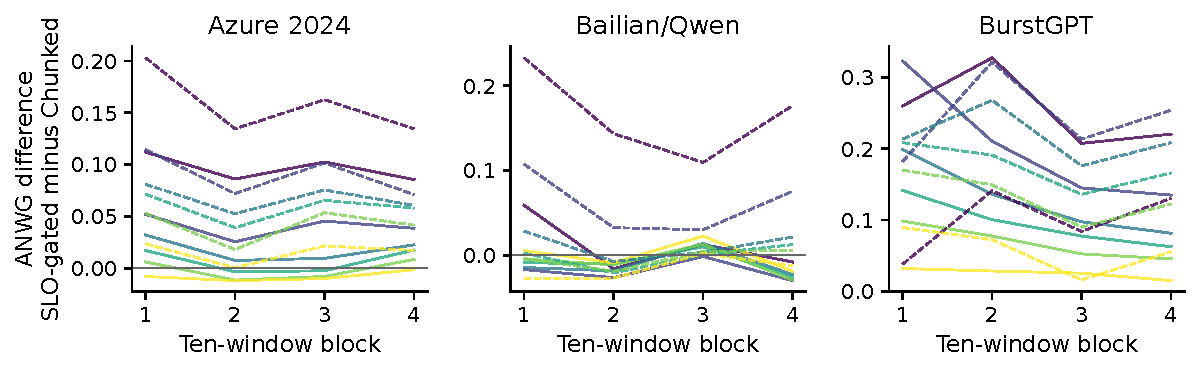
\includegraphics[width=\linewidth]{figures/chronology.pdf}
\caption{SLO-gated minus chunked-FCFS ANWG in four consecutive ten-window
blocks per source. Color advances from LOW (purple) to HIGH\_PRESSURE
(yellow); solid/dashed denotes four/eight residents. Each line fixes a
setting/capacity. Blocks are ordered corpus partitions, not equal-duration
or independent samples.}\label{fig:chronology}
\Description{Three panels plot all twelve setting/capacity series across
four blocks. Azure and Bailian include negative differences; BurstGPT
has positive differences throughout.}
\end{figure}

The supplement's \texttt{all-cell-metrics.csv} contains all 5,760 rows,
all accounting metrics and their condition, request, result and journal
hash references. \texttt{source-capacity-means.csv} retains all four
adaptations and all eleven ranking endpoints.
\texttt{matched-window-differences.csv} and
\texttt{chronological-differences.csv} contain the exact displayed
values. All six reversal axes and every exact/near-tie count are supplied
as CSV tables. Original per-setting source means, ranks and detailed
reversal groups remain in the hash-verified saved JSON reports.

\FloatBarrier
\section{Statistical Diagnostic Definitions and Full Scenario Accounting}\label{app:stat}
\subsection{Known truth and method identities}
Each synthetic study contains $Y_{sjw}$ for three sources, eleven policies
and normally 40 windows per source. The final bounded scenario has 400
windows. Sources and successive studies are independent by construction;
within-study windows and policies can be dependent. Positive population
means define the strict practical alternative for source pair $(s,t)$ and
policy pair $(a,b)$ as
\begin{align}
 &(\mu_{sa}>1.1\mu_{sb}\ \land\ \mu_{tb}>1.1\mu_{ta})\nonumber\\
 &\quad\lor(\mu_{sb}>1.1\mu_{sa}\ \land\ \mu_{ta}>1.1\mu_{tb}).
\end{align}
Equality at the boundary is null. Sign truth instead tests whether the
two mean differences have opposite signs. The 165 hypotheses are
$\binom{3}{2}\binom{11}{2}$ overlapping contrasts, not independent studies.

The default generator has Gaussian innovations, noise scale 0.15 and
cross-policy correlation 0.5. Window covariance is IID, independent
five-window blocks with correlation 0.7, or AR(1) with coefficient 0.7.
Equal means are 0.5; stable/near-tie means are $0.5+0.01j$ and
$0.5+0.0002j$. Reversal cases swap policies 0/1 between sources 0/1 at
$0.5\pm\delta/2$, leaving other means 0.5. Small, medium and large
reversals use $\delta=0.03,0.10,0.30$; dependence, variance and missingness
reversals use 0.15. The practical boundary swaps 0.55 and 0.5. Exact ties
use perfectly shared policy noise. Unequal scales are $(0.08,0.25,0.15)$;
the mixed case combines standardized Gaussian, $t_5$ and lognormal
innovations. MCAR masks observe each policy/window independently with
probability 0.8; the selective null hides below-mean source-0/policy-0
and source-1/policy-1 outcomes. Bounded cases use IID standardized uniform
innovations, scale 0.08 and $\delta=0.30$, analytically within $[0,1]$.
No latent missing values are imputed into an analysis.

\begin{table}[t]\centering\small
\caption{Eight original procedure IDs, abbreviated in Table~\ref{tab:scenarios}.
All have nominal $\alpha=q=0.05$. Historical methods use point screening
and zero-effect bootstrap components; the other reversal procedures test
practical contrasts and account for both orientations.}\label{tab:statmethods}
\begin{tabularx}{\linewidth}{lX}\toprule
Code & Frozen procedure and scope\\\midrule
HS & \texttt{historical\_screened\_BH}: practical point screen, 2,000
bootstrap draws, max of two source tail fractions, screened-family BH,
both percentile intervals exclude zero.\\
HF & \texttt{historical\_full\_BH}: same screened p-values; untested values
set to one in the full 165-hypothesis family.\\
HB & \texttt{historical\_plus1\_BY}: plus-one tail adjustment and full-family
BY; component and selection limitations remain.\\
T & \texttt{iid\_t\_Holm}: paired practical-contrast Student tests;
Gaussian IID complete/MCAR samples.\\
CT & \texttt{cluster\_t\_Holm}: tests on completely observed five-window
cluster means; Gaussian independent clusters; fewer than two clusters abstains.\\
O & \texttt{oracle\_normal\_Holm}: known covariance of matched means;
Gaussian complete/MCAR samples, including specified dependence.\\
G & \texttt{group\_bootstrap\_BY}: centered bootstrap over nonoverlapping
five-window groups, retaining masks; no asserted finite-sample guarantee.\\
B & \texttt{bounded\_Hoeffding\_Holm}: independent bounded samples only;
abstains elsewhere.\\\bottomrule
\end{tabularx}
\end{table}

For the nonhistorical procedures, a directional reversal requires both
source components, giving the maximum of their one-sided p-values. The
two possible orientations are combined by $\min(1,2\min(p_1,p_2))$ before
full-family adjustment. The bounded procedure uses Hoeffding's inequality
\citep{hoeffding1963} for $Z=Y_a-1.1Y_b\in[-1.1,1]$, with component
$p=\exp[-2n\max(\bar Z,0)^2/2.1^2]$. Valid component assumptions are
essential; Holm or BY does not supply them.

An additional \texttt{legacy\_source\_screened\_BH} preserves the actual
historical code. Eight \texttt{exact\_} counterparts correspond one to one
to Table~\ref{tab:statmethods}. All nine are post-diagnosis additions;
none replaces an original result or drives its stopping rule. For ordered
finite probabilities, exact BH rejects through the largest rank satisfying
$p_{(i)}\le i\alpha/m$, BY uses $i\alpha/(mH_m)$ with rational
$H_m=\sum_{j=1}^m1/j$, and Holm rejects successively while
$p_{(i)}\le\alpha/(m-i+1)$, with $\alpha=1/20$
\citep{benjamini1995,benjamini2001dependency,holm1979}.

Historical bootstrap probabilities are reconstructed as $2k/2000$ only
when the frozen floating expression reproduces the saved value exactly.
Plus-one values are $\min(1,(2k+2)/2001)$; grouped-bootstrap values use
$\min(1,2k/2001)$ with $k\ge1$. Analytic probabilities are exact dyadic
representations of the saved finite binary64 numbers, not infinitely
precise analytic tails. Nonfinite or off-grid inputs are rejected; there
is no boundary tolerance. Exact comparisons use independent rational
adjusted-p oracles, while legacy tests execute SHA-verified historical
source and preserve its stable-sort/missingness behavior.

\subsection{Uncertainty, stopping and endpoint denominators}
For each independent study, $R$ is the number of discoveries, $V$ the
number false under a specified truth, and FDP is $V/\max(R,1)$. FDR is its
expectation, FWER is $P(V>0)$, and power is the true-discovery fraction
when alternatives exist. Both sign and practical truth are retained.
Ordinary diagnostic coverage concerns the predeclared source-0,
policy-0-minus-policy-1 mean difference. Selected-interval coverage is
separate and conditional on emitting intervals; unavailable intervals
remain missing. For example, cluster-t emits ordinary intervals in only
1,676/8,000 MCAR studies and 202/8,000 selective-null studies. In the IID
equal null, historical selected coverage is 0.123834 over 958 emitting
studies, compared with 0.941875 ordinary diagnostic coverage over 8,000.
These are not interchangeable denominators or pooled independent intervals.

The finite analysis looks are 500, 1,000, 2,000, 4,000 and 8,000 studies
per scenario. For a bounded study endpoint with sample variance $s^2$ and
available count $N\ge2$, the two-sided empirical-Bernstein half-width is
\begin{equation}
 b=\sqrt{\frac{2s^2\log(4/\delta)}{N}}
   +\frac{7\log(4/\delta)}{3(N-1)}.
\end{equation}
Bounds clip $\bar X\pm b$ to $[0,1]$; counts below two receive the full
interval. This follows the bounded independent-observation inequality
and its two-sided union accounting \citep{maurer2009}. Original summaries
allocate $\delta=0.05/(18\cdot8\cdot16\cdot5)$; expanded summaries allocate
$0.05/(18\cdot17\cdot16\cdot5)$ to every included method. Endpoint
independence is not required for that finite union bound. Conditional
coverage uses the IID emitted-study population and its available count.
For post-diagnosis methods the statement is conditional on the fixed
amended family; it does not protect arbitrary data-dependent method search.

Only the original eight methods determine stopping: required half-widths
are at most 0.025 for practical FDR, FWER and null rejection fraction,
0.03 for ordinary coverage and 0.08 for power when defined. Precision is
not a calibration verdict. Table~\ref{tab:scenarios} includes every scenario
and the actual final stop. Seven of its nine empirical-compatibility entries
are exact-tie cases; the other two are conservative bounded procedures.
Across all 144 original method/scenario cells there are 45 concerns,
74 inconclusive results, nine compatible-with-tolerance results and
16 outside-domain abstentions.

\begin{table}[t]\centering\small
\caption{Complete original-family scenario accounting. P: precision
objective met; M: maximum count with precision gaps. C: FDR lower bound
$>0.05$ or ordinary-coverage upper bound $<0.95$; E: FDR upper bound
$\le0.06$ and coverage lower bound $\ge0.94$; I: inconclusive; A: outside-domain
abstention. E permits conservative overcoverage and is not exact nominal
calibration. Abbreviations follow Table~\ref{tab:statmethods}.}
\label{tab:scenarios}
\begin{tabular}{lrrcccccccc}\toprule
Scenario & Studies & Stop & HS & HF & HB & T & CT & O & G & B \\ \midrule
0: IID equal null & 8,000 & P & C & I & I & I & I & I & C & A \\
1: IID stable null & 8,000 & P & I & I & I & I & I & I & C & A \\
2: IID near ties & 8,000 & P & C & I & I & I & I & I & C & A \\
3: Exact policy ties & 2,000 & P & E & E & E & E & E & E & E & A \\
4: Practical boundary & 8,000 & M & C & I & I & I & I & I & C & A \\
5: Small sign reversal & 8,000 & M & C & I & I & I & I & I & C & A \\
6: Medium reversal & 8,000 & M & C & C & I & I & I & I & C & A \\
7: Large reversal & 8,000 & M & I & I & I & I & I & I & C & A \\
8: Block null & 8,000 & M & C & C & C & C & I & I & C & A \\
9: Block reversal & 8,000 & M & C & C & C & C & I & I & C & A \\
10: AR null & 8,000 & M & C & C & C & C & C & I & C & A \\
11: AR reversal & 8,000 & M & C & C & C & C & C & I & C & A \\
12: Unequal variances & 8,000 & M & I & I & I & I & I & I & C & A \\
13: Mixed distributions & 8,000 & M & I & I & I & I & I & I & C & A \\
14: MCAR reversal & 8,000 & M & I & I & I & I & I & I & C & A \\
15: Selective null & 8,000 & M & C & C & C & C & I & C & C & A \\
16: Bounded, n40 & 8,000 & P & I & I & I & I & I & I & C & E \\
17: Bounded, n400 & 4,000 & P & I & I & I & I & I & I & I & E \\
\bottomrule\end{tabular}

\end{table}

The full supplement \texttt{stat-all-endpoints.csv} reports all 16
endpoints, means, available counts, Monte Carlo standard errors and bounds
for both families (7,200 summary rows). It retains the nine additions and
all unfavorable/inconclusive outcomes. The finite-sample justification
of an assumption-aligned method is distinct from passing a finite precision
screen. Under AR dependence, cluster-t ordinary coverage is 0.8600 in the
null and 0.864375 with reversal. Under block reversal, cluster-t practical
power is about $6.58\times10^{-6}$, covariance-oracle power 0.000296,
and grouped-bootstrap power zero. These cases illustrate why low FDR
alone is not sufficient evidence of a useful procedure.

\subsection{The original numerical boundary case}
At scenario 11, replicate 6628, hypothesis index 47, a screened BH family
has $m=43$ and the relevant rank is 43. Stored $p=0.05$ has binary64
representation \texttt{0x1.999999999999ap-5}. The frozen port evaluates
\texttt{.05*43/43} as 0.049999999999999996, excluding that entry; the
historical source evaluates \texttt{(43/43)*.05} as 0.05, including it.
The exact finite-bootstrap interpretation is $p=1/20$, on the inclusive
critical boundary. In contrast, an \emph{analytic} stored float 0.05 is
slightly greater than rational $1/20$ and would be excluded at that exact
boundary. These deliberately different definitions cannot be reconciled
by silently introducing a tolerance.

Regression tests retain the old referee's failure and independently test
legacy source, exact adjusted probabilities, equality and neighboring
representable values, ties, sorting, family sizes and missingness. The
pinned suite records 118 passing tests. The completed recovery independently
validated every batch; review checked all 5,360 inventories and final
moment summaries, plus 200 saved studies including this case. Thirty-one
original records differed from actual historical-source behavior in the
112,275-study reuse audit; none was discarded or overwritten. At final
aggregation, only the exact screened-BH counterpart changes endpoint
means relative to its original, by at most $8.56\times10^{-7}$; the other
seven exact counterparts have equal aggregate means. Aggregate equality
is not a claim that every rejection vector is equal. These small numerical
differences do not repair the larger calibration failures.

\FloatBarrier
\section{Artifact Identities and Verification Route}\label{app:artifact}
The accompanying \texttt{evidence/source-manifest.json} records source
paths, byte counts and full SHA-256 values for 27 saved artifacts used
in the manuscript. Compressed copies preserve the exact uncompressed
bytes. Its per-window input manifest supplies source files, hashes,
row coordinates, chronology, condition factors and request fingerprints;
there are no within-corpus row overlaps in that manifest.

C01-FULL run identity begins \texttt{167b9074e5711420}; its completion
marker is \nolinkurl{EXECUTION_AND_INDEPENDENT_CHECKS_COMPLETE}.
STAT01 recovery identity begins \texttt{061933a64e27da20}; its marker is
\nolinkurl{COMPLETE_WITH_ORIGINAL_PRECISION_GAPS}. The completed jobs are
1440402 and 1440206, respectively. Deployment roots and immutable
completion/analysis hashes are enumerated in the accompanying claim-to-evidence
report and the preserved final-results review. Their raw journals,
synthetic arrays, original records and secondary decisions remain separate
from the manuscript package's presentation tables.

Presentation scripts only read saved artifacts and recompute summaries;
they never call a scheduler or synthetic generator. The manuscript
verification checks coverage, hashes, numerical claims, citations and
build outputs. The prior full-record review independently reproduced
7,200 STAT01 summaries and all C01 analysis outputs; its scope and sampled
raw checks are retained rather than relabeled as fresh exhaustive replay.
Author confirmation of external access is still necessary before this
internal evidence chain can be offered as a reproducible public artifact.
